  \subsection{Group Research}


\begin{table}[H]
	\centering
    
    \begin{tabular}{|p{3.5cm}|p{10.3cm}|}
    
    \hline
    \textbf{\large{Actors}}  			& \tabitem Third Party 																\\
    \hline
    \textbf{\large{Goals}} 				& \ref{goal:user0};\\
    
    \hline
    \textbf{\large{Enter Condition}}	& There is no enter condition for this Use Case		\\
    
    \hline
    \textbf{\large{Events Flow}}		& \begin{enumerate}[leftmargin=0.5cm]
                                          	\item The \emph{Visitor}  accesses to the web site or application log in page
                                           
                                          \end{enumerate}
    										\\
    \hline
    \textbf{\large{Exit Condition}} 	& The user is registered in the \emph{TrackMe} System, and his account is added to they system. Now the users is able to use all the functionalities provided by the system. \\
    
    \hline
    \textbf{\large{Exception}} 			& The \emph{Visitor} cannot register himself because is already registered.\newline The \emph{Registered} user                                         is not able to sign in the System because the login data are wrong or if he did not confirmed  the confirmation email. \newline
    										If one of these problems occur, the system both on the web site and on the application shows a message error to the user, which is invited to re-insert their credentials or confirm the registration email.\\
    
    \hline
    
    
    \end{tabular}
	
\end{table}
\begin{figure}[H]
    \centering
    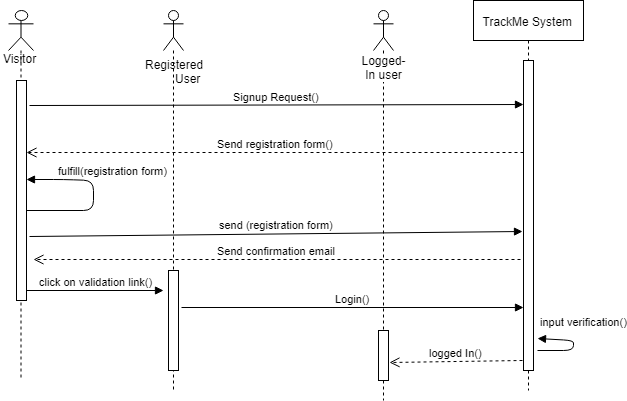
\includegraphics[scale=0.4]{rasdL/Pictures/login1.png}
    
\end{figure}
